\documentclass[10pt]{article}
\usepackage[margin=0.75in]{geometry}
\usepackage{amsmath,amssymb}
\usepackage{booktabs}
\usepackage{enumitem}
\usepackage{graphicx}
\usepackage[T1]{fontenc}
\usepackage[hidelinks]{hyperref}
\usepackage{caption}
\usepackage[expansion=false]{microtype}
\captionsetup{font=small,labelfont=bf,skip=2pt}
\setlist{nosep,leftmargin=1.2em}
\setlist[description]{style=unboxed,leftmargin=1.2em,labelindent=0pt,itemsep=1pt}
\graphicspath{{../results/}{../results/live_2026_10/}}
\setlength{\parskip}{2pt}
\setlength{\textfloatsep}{6pt}\setlength{\intextsep}{6pt}\setlength{\abovecaptionskip}{3pt}
\newcommand{\Fanon}{\mathcal{F}^{\mathrm{anon}}}
\newcommand{\Fid}{\mathcal{F}^{\mathrm{id}}}
\newcommand{\For}{\mathcal{F}^{\mathrm{oracle}}}
\newcommand{\LBR}{L_{\mathrm{BR}}}
\newcommand{\sect}[1]{\section*{\normalsize #1}\vspace{-2pt}}

\title{\vspace{-1.6em}{\Large\textbf{Rent or Toxicity? Strategic Exploitability of Learning Market Makers\\ with Public Wallet Information}}\\[0.15em]\large Wargame Deliverable 2 --- Workshop 1 report}
\author{Deepu Pradeep \quad Miguel Betran Menz\\
\normalsize 6.S974 Games, Learning, and Security --- Example 4 (Algorithmic Market with Adaptive Agents)}
\date{October 26, 2026}

\begin{document}
\maketitle
\vspace{-2.2em}

\sect{a) Setting and research questions}
\textbf{The contested system.} Hyperliquid is an on-chain exchange on which every order and both sides of every trade carry a persistent public wallet address, prices live on a coarse grid (five significant figures), standing orders at the same price are served first-in-first-out, and a protocol vault with undisclosed strategies supplies much of the resting liquidity. Market makers---increasingly learning algorithms---post standing prices; takers hit them; the difference between the price a maker gets and the asset's value afterwards is the maker's payoff. Three decisions matter: the makers' (how wide to quote, or, when the grid pins the quote, whether to keep an order standing); an adversary's (which of the makers' prices to undercut, or which fills to take); and the venue's (whether identities are public, how coarse the grid is, whether a place in the queue can be bought). The interaction is strategic in three ways. Independent learning makers settle on prices above the competitive level without communicating (tacit collusion): a \emph{rent}; but a wide price is also the correct charge for trading against better-informed takers (\emph{toxicity}), and the two look identical on the tape. An adversary must tell them apart, and its weapon---undercutting, or selecting the benign fills---is exactly what the makers' learned reaction function is tuned to punish. And the venue's information policy decides what the adversary and the defenders are allowed to know.

\textbf{Research questions and outcomes.} \textbf{RQ1 (value of identity):} what is public wallet identity worth to an entrant, over the anonymous tape, and through which mechanism? Outcome: $\pi^{\mathrm{id}}-\pi^{\mathrm{anon}}$ in rent units, as a function of regime persistence and the delay before outcomes become public; on data, whether the makers who earn condition on identity. \textbf{RQ2 (exploitability as measurement):} how much of a learned cartel's rent can an adversary take or destroy, and does more rent mean more vulnerability? Outcomes: the defenders' best-response loss $\LBR$, the fraction of rent destroyed $\kappa_A$, the adversary's profit, each against the rent index $C$; the exact best response; whether re-learning defends. \textbf{RQ3 (tick-constrained books and defences):} when the grid pins the price, where does rent live, and which venue and maker levers change who holds the toxic flow? Outcomes: realized spread per maker on Hyperliquid; in the queue game, the fill probability of uninformed takers in stress, venue revenue, and a profit--resilience frontier $(\mathbb{E}[\Pi_{\mathrm{nominal}}],\ \min_A\Pi_{\mathrm{attack}})$ for each lever.

\textbf{Changes since the proposal, and feedback.} The proposal's identity mechanism (a wallet's toxicity persists, so the last wallet predicts the next) is worth nothing on the data: same-wallet repeats are 2--5\% of orders. We replaced it with the mechanism the data support---informed flow clusters in time (a hidden regime) and a wallet's print reveals the regime before the price does (a mark lag)---and we added a second mode of the same environment, the one-tick queue game, after the book data showed the quoted spread never moves on the major pairs. RQ2 was reframed from a hypothesis to a measurement, and its headline changed when we computed the exact best response. Following the professor's feedback we define every market term once in the language of games and control (\S c), run one model in two modes rather than several, lead with results, and treat RQ1+RQ2 as the paper's spine with RQ3 built out as the project requires.

\sect{b) Literature and current practice}
\textbf{Algorithmic collusion.} Calvano et al.\ \cite{calvano} showed that independent Q-learners in a repeated pricing game converge to supra-competitive prices sustained by learned punishment; Colliard, Foucault and Lovo \cite{cfl} and Cont and Xiong \cite{cont} transplant this to market making in a Glosten--Milgrom \cite{gm} dealer market, where the wide quote has a second reading as the price of adverse selection; Cartea, Chang and Penalva \cite{ccp} show the tick grid itself sustains supra-competitive quotes; Dou, Goldstein and Ji \cite{dgj} study AI traders colluding through price impact. We take the environment and learners from \cite{cfl} and the mechanism test from \cite{calvano}. \textbf{Adversaries of learners.} Deng, Schneider and Sivan \cite{dss} and Brown and MacKay \cite{brownmackay} study a strategic player facing no-regret or algorithmic opponents and \emph{steering} their reaction functions; Gleave et al.\ \cite{gleave} show frozen RL policies are exploitable by adversaries that drive them off their training distribution; McMahan et al.\ \cite{mcmahan} and Lanctot et al.\ \cite{psro} give the double-oracle / PSRO loop. These are the attacker's side of RQ2; our exact best response is computed, not learned, because a frozen tabular cartel is a known reaction function. \textbf{Identity.} Zhai \cite{zhai} documents on Hyperliquid that public trader identity predicts adverse selection and returns; we turn that from a predictability fact into an information set and price it. \textbf{Data.} Albers et al.\ \cite{albers} publish the Hyperliquid L4 archive we use alongside our own recorder.

\textbf{Current practice (documented) vs.\ our assumptions.} Documented by the venue \cite{hldocs} and the archive \cite{albers}: wallet addresses on all orders and prints; price-time priority; a five-significant-figure price grid (one tick is $0.12$ / $0.39$ / $0.87$ / $0.11$\,bps on BTC/ETH/SOL/HYPE at current prices); per-address request budgets earned by filling; a priority mechanism for order placement; the HLP vault as a large resting liquidity provider whose strategy is not disclosed; liquidations routed to the book. How makers decide is not documented; what can be measured is the \emph{outcome}---which fills each wallet gets and what they earn---and \S d4 does that. Our modelling assumptions, all beyond documented practice: one unit traded per period at the best quote; takers of two types (informed / uninformed) drawn from a wallet population with persistent types under a hidden two-state regime; the asset value redrawn each period (so benchmarks are closed-form); tabular Q-learning incumbents with the state of \cite{cfl}; and, in the queue mode, a fixed one-tick spread with FIFO service. \textbf{What we add:} exploitability of learned cartels as a measured quantity (rules, then the exact best response and the double oracle); identity as a nested information set whose value is driven by regime persistence and the mark lag; the queue game with the venue's levers (anonymity, priority fee) and the makers' (speed, noise, identity-aware control) on one frontier; and three data anchors---the one-tick book, who earns the spread, and identity-conditioned fill selection by the makers who earn it.

\sect{c) Game formulation}
\textbf{Agents.} A \emph{venue} (chooses the rules once); $N$ \emph{incumbents} (defenders; $N\in\{2,3\}$); one \emph{entrant} (adversary); \emph{takers}, which are nature: a population of $M=50$ wallets with types $\alpha_j\in[0,1]$ (the probability wallet $j$'s order is informed), stratified quantiles of $\mathrm{Beta}(\bar\alpha\kappa_\alpha,(1-\bar\alpha)\kappa_\alpha)$ so the mean is $\bar\alpha$ and $\kappa_\alpha$ sets dispersion.

\textbf{State and uncertainty.} At period $t$: the fundamental $V_t=m_t\pm d_t$, $d_t\sim\mathrm{Exp}(\mu)$, redrawn each period around the public reference price $m_t$ (the \emph{mid}); a hidden regime $z_t\in\{\text{calm},\text{toxic}\}$ kept with probability $\rho_z$, else redrawn from a law with stationary mean toxicity $\bar\alpha$; last period's quote vector $h_{t-1}$; in the queue mode, the FIFO queue of standing orders. Wallet activity depends on the regime (toxic: arrival weight $\propto\alpha_j$; calm: $\propto1-\alpha_j$), so at $\kappa_\alpha=1$ the two states have toxicity $0.15$ and $0.65$ around $\bar\alpha=0.3$: \emph{who just traded is evidence about the state the next trader shares}.

\textbf{Actions.} Spread mode: each maker posts a half-spread $h\in\{1,\dots,K\}$ ($K=24$, tick $\theta=0.5$), i.e.\ offers to sell at $m_t+h\theta$ and buy at $m_t-h\theta$. Queue mode: the spread is pinned at $h$ and each maker chooses \textsc{rest} (keep a standing order at the inside), \textsc{out}, or \textsc{rest-and-pay} (the venue's priority fee $f$ per period, served ahead of non-payers). Venue levers: identity public or not, the tick, the fee. Resource constraints: one unit per fill, an inventory cap (never binding in the reported runs), and the venue's request budget (modelled as the fee's cost, not as rate limiting, so far).

\textbf{Information.} Incumbents (tabular Q-learners, state $=$ own last $h$ and the best rival's last $h$) are identity-blind by construction. The entrant's information set is a treatment: $\Fanon$ (the public tape: every print's event, price, and its mark $L$ periods later) $\subset\Fid$ ($+$ the wallet on every print) $\subset\For$ ($+$ the regime). On $\Fid$ the entrant runs a Bayesian filter: wallet-type posteriors from fills and a regime belief from the sequence of wallets, giving $\alpha_{\mathrm{next}}$, the implied probability that the next taker is informed; on $\Fanon$ the same filter sees only outcomes, which arrive $L$ periods late.

\textbf{Sequence of play (one period).} (1) Makers commit actions simultaneously. (2) Nature draws the regime, then a wallet, then whether its order is informed. (3) The taker hits the best quote: an informed taker trades iff the quote is strictly inside $V_t$ (so it only trades when the maker loses); an uninformed one trades iff a private valuation $m_t+\mathcal{N}(0,\sigma_L^2)$ crosses it. One unit goes to a maker at the best quote (random tie split in spread mode; the front of the queue in queue mode, which then rejoins at the back). (4) The print (event, price, wallet) becomes public; its mark $V_t$ becomes public at $t+L$. (5) Payoffs: the filled maker earns $\pm(\text{price}-V_t)$, minus the fee if paying; the venue collects fees. Horizon: $T=100$ periods per episode; episodes are a training device, the wallet population and regime chain persist across them. Training: $2\times10^4$ episodes; evaluation: 300--500 episodes with the incumbents frozen (greedy), under common random numbers across treatments.

\textbf{Payoffs and benchmarks (closed form).} The market-wide expected one-period payoff of a best quote $h$ against informed share $\alpha$ is $\Pi(h;\alpha)=(1-\alpha)\,2x\bar\Phi(x/\sigma_L)-\alpha\mu e^{-x/\mu}$, $x=h\theta$ ($\sigma_L=8$, $\mu=5$); the makers at the best quote split it. $h^C=\min\{h:\Pi\ge0\}$ is the Nash point of the one-shot game (any $h>h^C$ is undercut), $h^M=\arg\max_h\Pi$ the joint monopoly; $(h^C,h^M)=(2,13),(4,14),(8,17)$ and $\Pi^M-\Pi^C=1.90,1.38,0.66$ at $\bar\alpha=0.1,0.3,0.5$. The \emph{rent index} $C(\pi)=(\Pi_{\mathrm{nominal}}-\Pi^C)/(\Pi^M-\Pi^C)$ places a frozen profile between Nash (0) and monopoly (1). With adversary $A$ present the defenders earn $J(\pi;A)$; $\LBR^A=\Pi_{\mathrm{nominal}}-J$ is their loss, $\kappa_A=\LBR/(\Pi_{\mathrm{nominal}}-\Pi^C)$ the fraction of rent destroyed, and ``rent units'' divide by $\Pi^M-\Pi^C$. The game is general-sum: the defenders' loss, not the adversary's gain, is the statistic. \emph{Small example} ($\bar\alpha=0.3$): two incumbents at $h=14$ split $\Pi(14)=1.50$; an entrant at $13$ takes every fill and earns $\Pi(13)=1.49$ alone, the incumbents earn 0; if they answer by moving to $12$, the entrant at $11$ earns $1.39$; the chase ends at $h^C=4$ where $\Pi=0.12$. A learned cartel is a reaction function that does \emph{not} chase every time.

\textbf{Why this structure.} One unit per period and an i.i.d.\ value give closed-form benchmarks, so rent is measured, not estimated; the grid and the FIFO queue are the venue's documented rules; tabular Q-learners are the incumbents of the literature we replicate; the regime and the mark lag are what the data forced on us. Everything else is held fixed so treatments differ in one thing.

\sect{d) Preliminary results}
\textbf{d1. Learners coordinate above the Nash point.} Two or three Q-learners settle at $10.6$, $14.4$, $17.4$ ticks at $\bar\alpha=0.1,0.3,0.5$ against Nash $2,4,8$ and monopoly $13,14,17$: $C=0.83,0.86,0.77$ (seed sd $0.01$--$0.02$), replicating \cite{cfl}; a grid over $N\in\{2,3,5\}$, learning rate and initialisation gives $C=0.71$--$0.87$ in every cell. The mechanism is restraint: in 55--83\% of visited states a rival sits at or inside the monopoly quote, and in 96--100\% of those the learner's greedy action forgoes the undercut. Fills rotate (no leader); an undercut shock is answered in kind and the cartel re-forms within a few periods.

\textbf{d2. Exploitability.} \emph{Rule adversaries} (180 frozen populations, $C\in[0.42,0.97]$, four adversaries, 500 episodes): the literal hypothesis $\partial\LBR/\partial C>0$ holds by construction (the competitive quoter pushes the cartel below $\Pi^C$, slope $1.03\,[1.00,1.07]$), but the substantive one does not: $\kappa_A$ is $0.71$--$0.73$ for the undercutter, the markout entrant (infers toxicity from its own fills) and the oracle, flat in $C$. The markout entrant keeps 79--96\% of the monopoly rent and keeps it when the incumbents re-learn: the cartel re-forms around it. \emph{The exact best response} (Figure~\ref{fig:br}, 60 cartels). A frozen cartel is a deterministic reaction function with known transitions and closed-form rewards, so the entrant's problem is a finite-horizon MDP solved exactly by backward induction for any objective $\lambda\cdot\text{own}-(1-\lambda)\cdot\text{incumbents}$ (DP and simulation agree to $0.02$). It takes everything: $\LBR>C$ in 60 of 60 cartels, the entrant earns $1.08$--$1.20$ rent units---the monopoly profit itself---and $\kappa_A=1.14$--$1.29$; the rules reach 55--70\% of it. How: it undercuts the \emph{reaction}, not the last print (one tick inside what the incumbents are about to quote, 100\% of periods), and holds the cartel at $Q$-cells it never visits on its own path (86--99\% of periods), where the learned response sends it \emph{wider}---$10.8\to15.9$ ticks at $\bar\alpha=0.1$, $17.8\to21.9$ at $0.5$. The damage-maximiser ($\lambda=0$) steers the cartel \emph{tight}, to 4--7 ticks inside break-even, by quoting above it, takes no fills, earns nothing, and leaves the incumbents absorbing toxic flow at losing quotes: $\LBR=1.3$ at $\bar\alpha=0.3$, $2.7$--$2.8$ at $0.5$---two to three times the rent, at no cost. \emph{Double oracle:} letting the cartel re-learn 3000 episodes against the best response and re-solving, three rounds, re-learning buys back about half of a stale attacker's take (its profit $1.2\to0.5$) and nothing against the re-solved one ($\LBR\ge0.9C$ in every cartel every round), while the cartel's own rent erodes $0.83\to0.69$. \emph{Robustness:} cartels keep $C=0.80$--$0.86$ and $\kappa_A=0.65$--$0.75$ (rules) on any market calmer than the one they trained on; on a more toxic one their rent collapses ($C=0.23$ for the $0.1$-cartel at $0.5$) and is more than destroyed; held-out adversaries preserve every ordering (Spearman $0.75$--$0.96$).

\begin{figure}[t]\centering
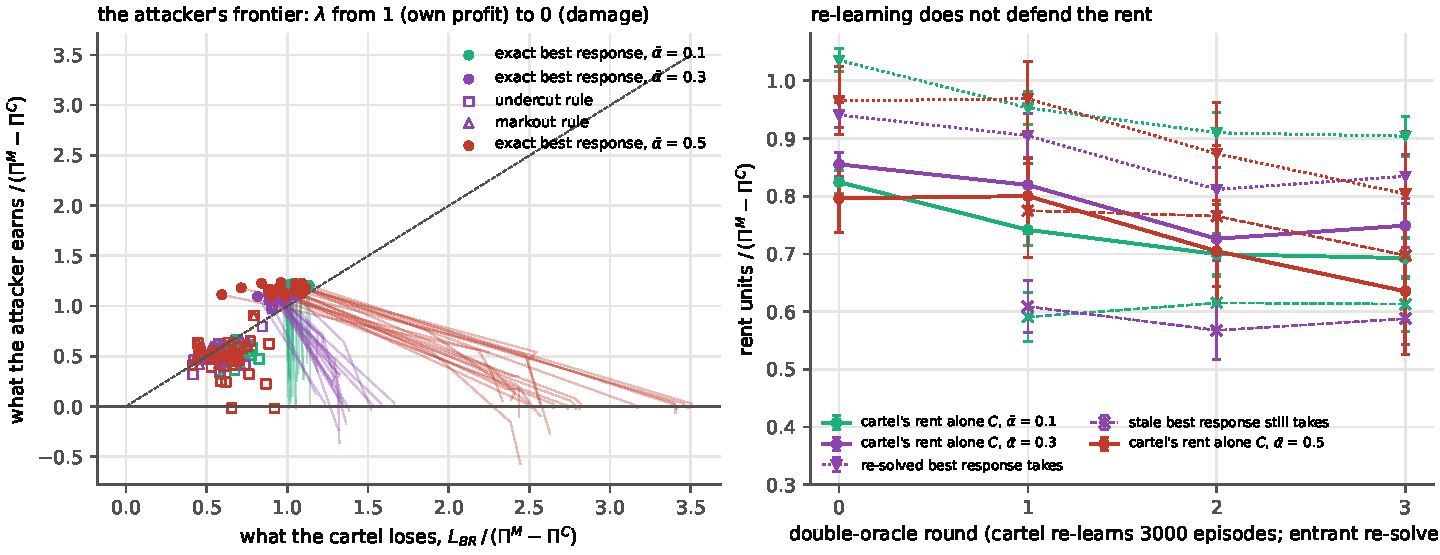
\includegraphics[width=0.88\textwidth]{fig_best_response.pdf}
\caption{Left: each cartel's attacker frontier (rent units) from $\lambda=1$ (own profit) to $0$ (damage); hollow markers: the hand-crafted rules; diagonal: $\kappa_A=1$. Right: the double oracle; mean and 95\% interval over ten seeds.}\label{fig:br}
\end{figure}

\textbf{d3. What identity is worth in the simulator (RQ1).} Under the proposal's mechanism identity is worth $+0.15$ to $+0.30$ rent units when wallets repeat ($\rho=0.9$--$0.99$) and exactly zero when they do not---and on Hyperliquid they do not. Under the regime mechanism with the mark revealed immediately ($L=1$) identity adds only $+0.03$ to $+0.06$: the last print's \emph{outcome} is as good a regime signal as its author. With the lag, the anonymous entrant's profit falls as the mark arrives later while the identity entrant's does not, so the increment grows from $+0.06$ to $+0.16$ ($\pm0.07$) at $\bar\alpha=0.5$, $\rho_z=0.99$, and peaks at $L=20$ for $\rho_z=0.9$, where a regime lives about ten arrivals: identity's value grows with the lag up to the regime's lifetime, and is zero where the toxic state still leaves an undercut profitable ($\bar\alpha\le0.3$ against 11-tick cartels). At $\kappa_\alpha=5$ it can hurt: three of ten cartels punish the informed entrant's moving quote and the naive undercutter out-earns it---the reaction function is part of the game, which d2 then exploits.

\textbf{d4. Hyperliquid data (Table~\ref{tab:data}, Figure~\ref{fig:idsel}).} Two top-of-book recording sessions eight days apart (15 h, 300k marked fills) and 327 h of signed trades. \emph{The price cannot move:} the quoted spread on BTC/ETH/SOL is one tick essentially always (p90 $=$ median). A fill at the touch pays exactly that tick and loses $0.3$--$0.6$\,bps to the mid within ten seconds on every coin; the taker's cost is in depth (one order in ten walks the book and pays twenty ticks, and on the deep books those are the informed ones). \emph{Someone still earns the spread:} the ten most active market-maker wallets (chosen on activity, scored on outcome) break even or earn where everyone else loses; at the same price they earn $0.4$--$1.1$\,bps per fill more, and their ranking persists night to night (Spearman $0.43$--$0.75$, $p<10^{-3}$). \emph{How: identity, not the tape.} They never withdraw from the touch after a stressful spell at any timescale (30 s to 5 min blocks, or the mid's move in the 10 s before each fill: correlations $-0.07$ to $+0.13$). But typing every taker on night 1 by the toxicity it inflicted and scoring night 2, the top makers take $0.03$ / $0.06$ / $0.12$ / $0.12$ of last night's toxic wallets' fills against $0.12$ / $0.38$ / $0.42$ / $0.30$ of the benign ones (BTC/ETH/SOL/HYPE; $2.6$--$6.5\times$, $p<10^{-3}$), the same gap inside calm and stressed tape, and still $1.3$--$2.8\times$ on fills after which the mid did not move within a second (not pick-offs). The typing holds (toxic wallets cost $1.0$--$2.3$\,bps more on night 2). Identity-conditioned fill selection is operating on the real book: RQ1's mechanism, observed.

\begin{table}[t]\footnotesize\centering
\resizebox{0.98\linewidth}{!}{%
\begin{tabular}{lcccc}
\toprule
 & BTC & ETH & SOL & HYPE \\
\midrule
quoted spread median / one tick (bps) & 0.12 / 0.12 & 0.39 / 0.39 & 0.90 / 0.86 & 0.12 / 0.11 \\
effective spread: at the touch / walked / per order (bps) & 0.12 / 2.35 / 0.27 & 0.42 / 3.20 / 0.60 & 0.92 / 5.20 / 1.09 & 0.17 / 3.57 / 0.40 \\
10-s maker markout, at the touch / walked (bps) & $-0.41$ / $-0.80$ & $-0.56$ / $-2.26$ & $-0.27$ / $+0.98$ & $-0.45$ / $-0.01$ \\
after a toxic vs a benign wallet, given the anonymous signal (bps, 327 h) & $-0.64$ & $-1.01$ & $-0.59$ & $-0.59$ \\
at the touch: top-10 MM / everyone else (bps) & $-0.02$ / $-0.41$ & $+0.24$ / $-0.70$ & $+0.52$ / $-0.56$ & $+0.09$ / $-0.56$ \\
per-maker rank correlation, night vs night ($n$ makers) & 0.75 (108) & 0.50 (65) & 0.56 (45) & 0.43 (68) \\
top-10 share of touch fills: benign / unseen / toxic wallets & .12 / .13 / .03 & .38 / .31 / .06 & .42 / .39 / .12 & .30 / .25 / .12 \\
\bottomrule
\end{tabular}}
\caption{Hyperliquid, Oct.\ 2026. SEs cluster by five-minute block; every top-10-vs-rest gap exceeds four SEs. Wallet types from night 1, scored on night 2.}\label{tab:data}
\end{table}

\begin{figure}[t]\centering
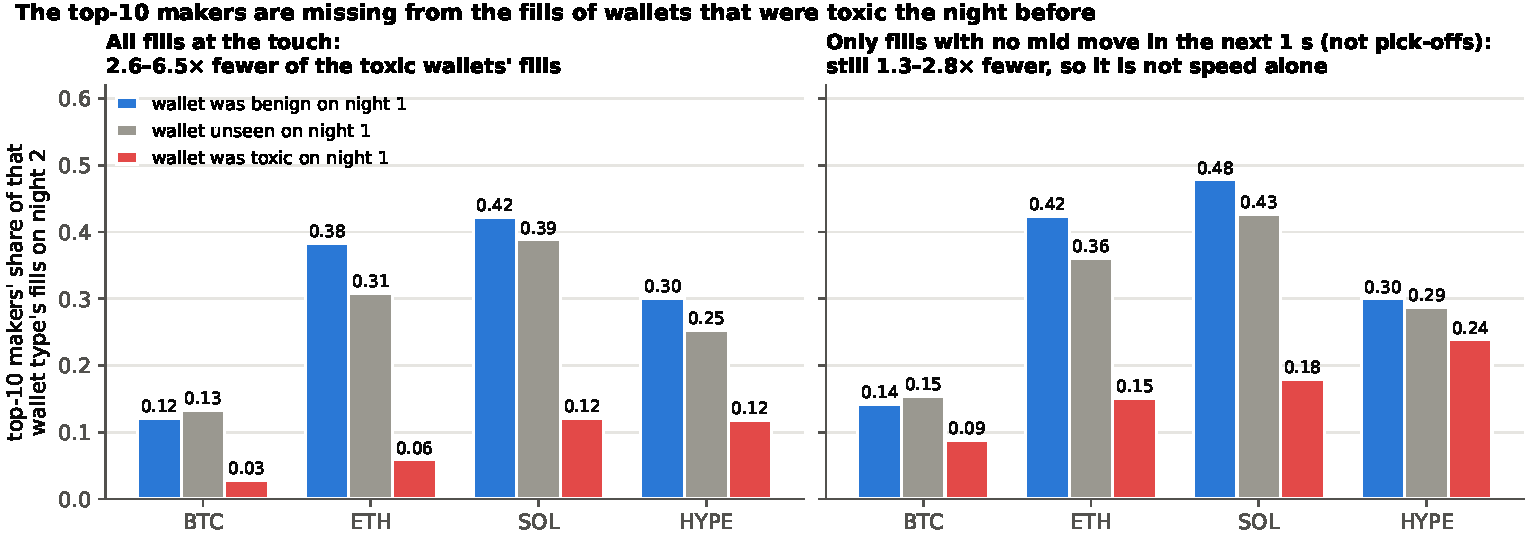
\includegraphics[width=0.84\textwidth]{fig_identity_selection.pdf}
\caption{Identity selection on the book: top-10 makers' share of fills at the touch on night 2 by the taker's type on night 1; lighter bars keep only fills after which the mid did not move within 1\,s. Dashed: their share of all touch fills.}\label{fig:idsel}
\end{figure}

\textbf{d5. When the price cannot move: the queue game and the levers (RQ3).} With the spread pinned at $h^C$ a fill is worth $+0.15$ on average, $+1.10$ in the calm state and $-2.26$ in the toxic one: all value is in selection. Against always-resting incumbents the identity entrant earns $0.14$--$0.16$ per period by resting only when the forecast is calm (its fills 16\% informed vs the incumbents' 29--31\%) and its edge over the tape-reading entrant grows with the lag ($+0.04\to+0.10$). Incumbents that learn need a \emph{fringe} of always-resting makers (else a toxic spell empties the book and locks it), and tabular Q cannot learn to queue (time priority pays only after consecutive periods in line); no-regret (EXP3) incumbents over complete policies converge in a few hundred episodes, learn to select, and identity is then worth \emph{more}, $+0.05$ to $+0.06$ at every lag, five of five seeds---while the fringe's payoff goes from $\approx0$ to $-0.02$ to $-0.10$: identity-blind resting liquidity is the counterparty of the selection rent, in the simulator as on the book. \emph{Venue levers.} Anonymity with a stale tape keeps incumbents resting in the toxic state (an uninformed taker is filled 71--75\% of the time, the incumbents earn $\approx0$); identities let them withdraw (fill probability $0.23$--$0.30$, incumbents earn $0.12$--$0.14$), and an identity-blind maker among them earns $-0.13$ to $-0.29$. Anonymity is a transfer from makers to uninformed takers in stress; neither setting defends the rent. The priority fee is an all-pay auction for position: at the venue's revenue-maximising $f=0.5$ it collects two to four times the makers' total rent and leaves every maker at or below zero; a cheap fee doubles the best-informed's profit; the fringe's loss triples at any fee. \emph{Makers' levers} (20 cartels, seven adversaries incl.\ a learned one): requoting slowly costs everything ($\kappa_A\to1.0$--$1.3$); noise costs profit and buys nothing; flooring the quote at the identity forecast's break-even is the only lever that improves both profit and resilience, and only where the toxic regime bites ($\bar\alpha=0.5$: worst-case profit $0.08\to0.19$). It still leaves the rule adversary 75--80\% of its take. Nothing in the game defends the rent; the levers decide who holds the toxic flow.

\textbf{Limitations.} The exact best response uses the cartel's reaction function (oracle knowledge of the \emph{policy}); it is the true upper bound, and the realistic attacker that identifies the function from public quotes is not yet built (\S f). Incumbents are tabular and frozen at evaluation; the double oracle is three rounds. Data: two nights, four pairs; wallet types need $\ge30$ fills, so the typed set is the active takers; a cross-venue price lead is not excluded as the top makers' signal on pick-offs (it cannot produce the quiet-fill gap). The simulator trades one unit at the best quote, so depth---where the data put the taker's cost---is not modelled.

\sect{e) Prototype}
\textbf{State.} A Python package (\texttt{github.com/pradeepu191/wargame}; 59 tests): \texttt{sim/} (the environment with wallets, regime and mark lag; Q-learners and frozen incumbents; rule adversaries and the wallet entrant's Bayesian filter on $\Fanon$/$\Fid$/$\For$; the queue mode with FIFO, fee and EXP3 incumbents; closed-form benchmarks), \texttt{experiments/} (training sweeps, entry, exploitability, identity grids, queue game, defences, exact best response and double oracle), \texttt{analysis/} (recorder, true-mid markouts, per-maker realized spread, stress and identity selection), SLURM scripts, and \texttt{results/REPLICATION\_NOTES.md}, a log of every result with its command. \textbf{How it operates.} \texttt{python experiments/demo.py} runs a small instance in seconds: it prints the benchmarks ($h^C=4$, $h^M=14$, $\Pi(h)$), plays the shipped two-maker cartel alone ($C=0.86$), enters three adversaries under common random numbers (undercut: cartel loses $0.41$, entrant earns $0.33$; markout: $0.47/0.41$; exact best response: $0.94/1.09$, $\kappa_A=1.10$), and traces ten periods of the best response: \\[1pt]
{\footnotesize\texttt{\ t\ \ inc0\ inc1\ entrant\ \ taker\ \ \ \ \ \ \ \ \ filled\ \ payoff}\\
\texttt{\ 0\ \ \ 15\ \ \ 24\ \ \ \ \ \ 12\ \ noise\ \ \ \ buy\ \ entrant\ \ +1.21}\\
\texttt{\ 5\ \ \ 21\ \ \ 19\ \ \ \ \ \ 14\ \ informed\ buy\ \ entrant\ \ -5.77}\\
\texttt{\ 7\ \ \ 18\ \ \ 23\ \ \ \ \ \ 14\ \ noise\ \ \ \ buy\ \ entrant\ +11.79}}\\[1pt]
The incumbents answer each entrant quote with their learned reaction; the entrant sits one tick inside what they are about to quote and holds them where they never trained. \texttt{--train} fits a fresh cartel first (two minutes; $C=0.83$, best response takes $0.91$). The implementation is \S c line by line: the period's sequence is \texttt{env.step}, an information set is what an agent's \texttt{act} may read from the observation, and the benchmarks are the closed form quoted above. \textbf{Remaining:} the public-information attacker (\S f); learned entrants and re-learning cartels in one PSRO loop; depth as an action; the request budget as a resource constraint; a replay harness scoring a policy on recorded fills.

\sect{f) Plan for Workshop 2}
\textbf{Modelling and implementation.} (1) \emph{The attacker with public information only}: a model-based entrant on $\Fanon$ that identifies each incumbent's reaction function from the tape (every answer to (own, rival) is a public print, and the entrant sets ``rival'' with its own quote) and solves the identified MDP; the number to report is its gap to the exact best response against the probing budget. (2) \emph{Both sides learning}: PSRO with re-learning cartels and learned entrants---the equilibrium's rent and $\kappa_A$, and whether adversarially trained cartels are less exploitable or just less collusive. (3) \emph{Queue-mode attacks}: steering no-regret incumbents' weights; the request budget as a drainable resource. (4) \emph{Resilient designs}: venue levers---anonymity, tick, fee, request allowance---and maker levers, each reported on the frontier $(\mathbb{E}[\Pi_{\mathrm{nominal}}],\ -\mathrm{CVaR}_{0.05}(\Pi_{\mathrm{attack}}))$ against the three attackers (profit-maximiser, damage-maximiser, public-information learner), plus the uninformed takers' fill probability in stress, so ``robust'' cannot mean ``withdrew''. \textbf{Data.} An always-on recorder (weeks of top-of-book: the identity-selection gap by coin, hour and regime, with intervals); the October 2025 liquidation cascade as the stress case; the December 2025 order lifecycles to say which \emph{action}---cancellation, queue position, depth---carries the selection the prints show. \textbf{Evaluation throughout:} common random numbers, paired-per-seed intervals, CVaR alongside means, train-at-$\bar\alpha$/test-at-$\bar\alpha'$, held-out adversaries, chronological splits. Preprint by mid-December.

\begin{thebibliography}{9}\footnotesize\setlength{\itemsep}{0pt}
\bibitem{gm} L. R. Glosten, P. R. Milgrom. Bid, ask and transaction prices in a specialist market with heterogeneously informed traders. \emph{J.\ Financial Economics} 14, 1985.
\bibitem{calvano} E. Calvano, G. Calzolari, V. Denicol\`o, S. Pastorello. Artificial Intelligence, Algorithmic Pricing, and Collusion. \emph{AER} 110(10), 2020.
\bibitem{cfl} J.-E. Colliard, T. Foucault, S. Lovo. Algorithmic Pricing and Liquidity in Securities Markets. \emph{Review of Financial Studies}, 2026.
\bibitem{cont} R. Cont, W. Xiong. Dynamics of market making algorithms in dealer markets: learning and tacit collusion. \emph{Mathematical Finance} 34(2), 2024.
\bibitem{ccp} \'A. Cartea, P. Chang, J. Penalva. Algorithms and Supracompetitive Prices in Electronic Markets: The Impact of Tick Size. SSRN 4105954, 2026.
\bibitem{dgj} W. W. Dou, I. Goldstein, Y. Ji. AI-Powered Trading, Algorithmic Collusion, and Price Efficiency. NBER WP 34054, 2025.
\bibitem{dss} Y. Deng, J. Schneider, B. Sivan. Strategizing against No-Regret Learners. \emph{NeurIPS} 2019.
\bibitem{brownmackay} Z. Y. Brown, A. MacKay. Competition in Pricing Algorithms. \emph{AEJ: Microeconomics} 15(2), 2023.
\bibitem{gleave} A. Gleave, M. Dennis, C. Wild, N. Kant, S. Levine, S. Russell. Adversarial Policies: Attacking Deep Reinforcement Learning. \emph{ICLR} 2020.
\bibitem{mcmahan} H. B. McMahan, G. J. Gordon, A. Blum. Planning in the Presence of Cost Functions Controlled by an Adversary. \emph{ICML} 2003.
\bibitem{psro} M. Lanctot et al. A Unified Game-Theoretic Approach to Multiagent Reinforcement Learning. \emph{NeurIPS} 2017.
\bibitem{zhai} D. Zhai. Public Trader Identity: Adverse Selection and Return Predictability. arXiv:2608.04373, 2026.
\bibitem{albers} J. Albers, M. Cucuringu, S. Howison, A. Y. Shestopaloff. An Open Book: Level 4 Order Book Data from the Hyperliquid Exchange. SSRN 6465720, 2026.
\bibitem{hldocs} Hyperliquid Documentation. \url{https://hyperliquid.gitbook.io/hyperliquid-docs}, accessed Oct.\ 2026.
\end{thebibliography}
\end{document}
